\documentclass[11pt,letterpaper]{article}

% Load some basic packages that are useful to have
% and that should be part of any LaTeX installation.
%
% be able to include figures
\usepackage{graphicx}
% get nice colors
\usepackage{xcolor}

% change default font to Palatino (looks nicer!)
\usepackage[latin1]{inputenc}
\usepackage{mathpazo}
\usepackage[T1]{fontenc}
% load some useful math symbols/fonts
\usepackage{latexsym,amsfonts,amsmath,amssymb}

% comfort package to easily set margins
\usepackage[top=1in, bottom=1in, left=1in, right=1in]{geometry}

% control some spacings
%
% spacing after a paragraph
\setlength{\parskip}{.15cm}
% indentation at the top of a new paragraph
\setlength{\parindent}{0.0cm}


\begin{document}

\begin{center}
\Large
Ay190 -- Worksheet 2\\
Scott Barenfeld\\
Date: \today
\end{center}

This week, I worked with Daniel DeFelippis and Donal O'Sullivan.

\section{Problem 1}
The values for the recurrence relation and exact relation are shown in 
Table \ref{tab:one}.  For $n=15$, the absolute error is 3.66 and the 
relative error is $5.25\times10^{7}$.

\begin{table}[!h]
\centering
\caption{Problem 1 recurrence relation}
\begin{tabular}{c|c}
\hline
Recurrence Relation & Exact Relation\\
\hline
\hline
1.00 & 1.00\\
0.33 & 0.33\\
0.11 & 0.11\\
3.70$\times$10$^{-2}$ & 3.70$\times$10$^{-2}$\\
1.23$\times$10$^{-2}$ & 1.23$\times$10$^{-2}$\\
4.12$\times$10$^{-3}$ & 4.12$\times$10$^{-3}$\\
1.39$\times$10$^{-3}$ & 1.37$\times$10$^{-3}$\\
5.13$\times$10$^{-4}$ & 4.57$\times$10$^{-4}$\\
3.76$\times$10$^{-4}$ & 1.52$\times$10$^{-4}$\\
9.44$\times$10$^{-4}$ & 5.08$\times$10$^{-5}$\\
3.59$\times$10$^{-3}$ & 1.69$\times$10$^{-5}$\\
1.43$\times$10$^{-2}$ & 5.65$\times$10$^{-6}$\\
5.72$\times$10$^{-2}$ & 1.88$\times$10$^{-6}$\\
0.23 & 6.27$\times$10$^{-7}$\\
0.91 & 2.09$\times$10$^{-7}$\\
3.66 & 6.97$\times$10$^{-8}$\\
\hline
\end{tabular}
\label{tab:one}
\end{table}

\section{Problem 2}
Figure \ref{fig:two} shows the absolute error in computing the 
derivative of 
\begin{equation}
f(x)=x^3-5x^2+x
\end{equation}
using forward differencing.  Figure \ref{fig:two2} shows the 
absolute error if central differencing is used.  The error in 
forward differencing goes as $h$, so halfing $h$ should half the error.  
To show this, half the value of the $h=0.1$ absolute is plotted in Figure 
\ref{fig:two} with crosses.  It matches up almost exactly with the 
absolute error for $h=0.05$, as it should.  Similarly, Figure 
\ref{fig:two2} shows $1/4$ of the $h=0.1$ absolute error, since 
central differencing error goes as $h^2$.  This also matches almost 
exactly.

Since both schemes really 
on surrounding points to calculate the derivative, the derivative is 
not calculated at $x=6$ for forward differencing or for $x=-2$ and 
$x=6$ for central differencing.

\begin{figure}
\centering
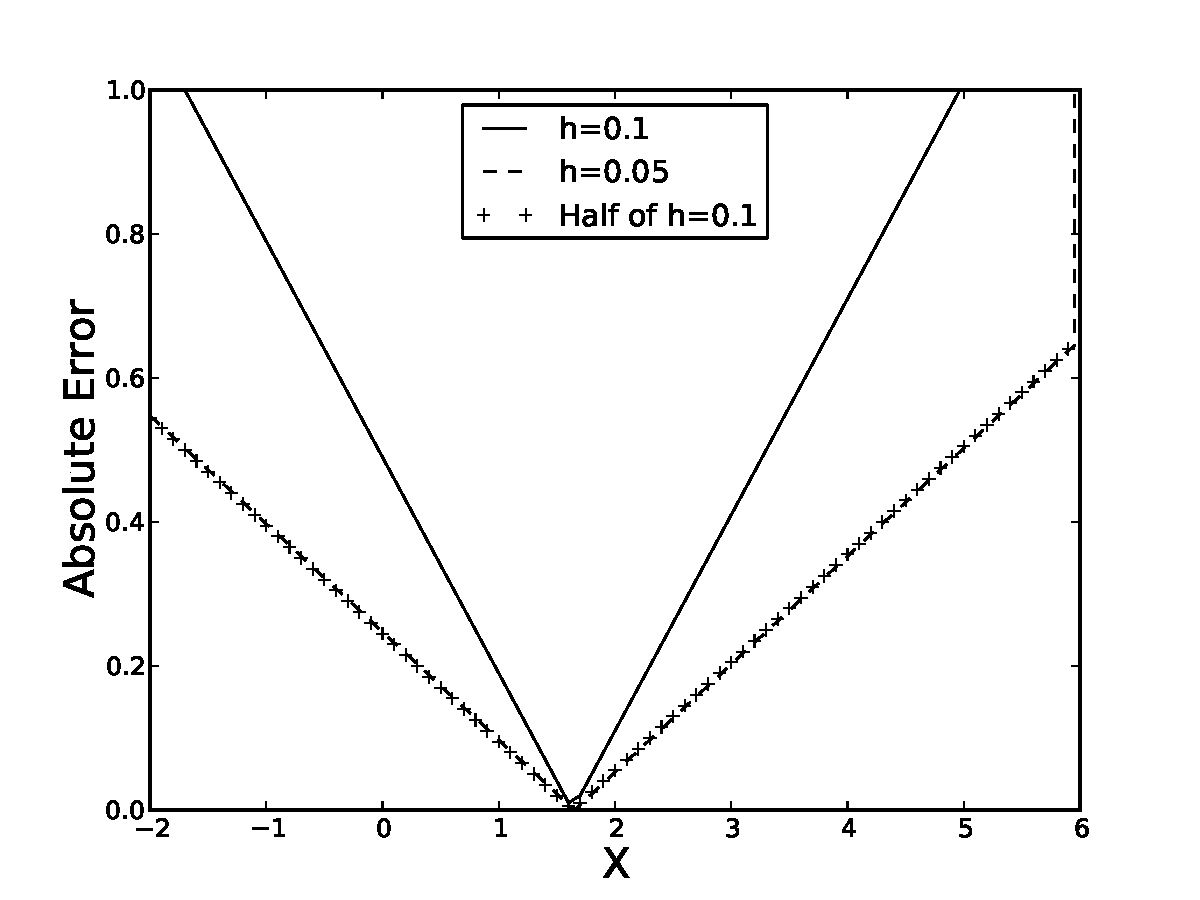
\includegraphics[width=0.5\textwidth]{twoi.pdf}
\caption{Absolute error of forward differencing.  The solid line shows 
the absolute error for h=0.1.  The dashed line shows absolute error 
for h=0.05.  Half of the h=0.1 absolute error is plotted with crosses, 
as discussed in the text.}
\label{fig:two}
\end{figure} 

\begin{figure}
\centering
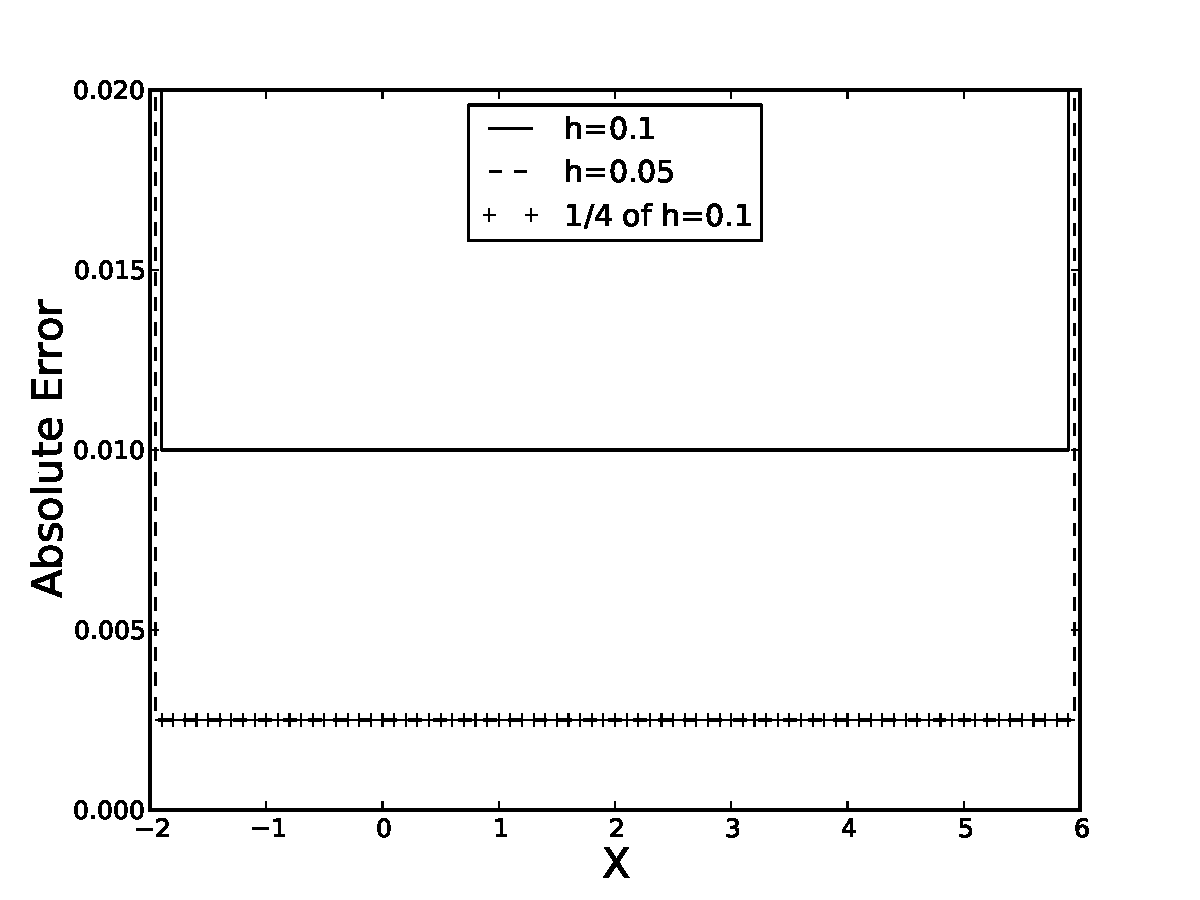
\includegraphics[width=0.5\textwidth]{twoii.pdf}
\caption{Absolute error of central differencing.  The solid line shows 
the absolute error for h=0.1.  The dashed line shows absolute error 
for h=0.05.  One quarter of the h=0.1 absolute error is plotted with crosses, 
as discussed in the text.}
\label{fig:two2}
\end{figure} 

\section{Problem 3}
Start with the Taylor expansion of $f(x_0+h)$:
\begin{equation}
f(x_0+h)=f(x_0)+hf'(x_0)+\frac{h^2}{2}f''(x_0)+\frac{h^3}{6}f'''(x_0)+\mathcal{O}(h^4)
\end{equation}
and of $f(x_0-h)$:
\begin{equation}
f(x_0-h)=f(x_0)-hf'(x_0)+\frac{h^2}{2}f''(x_0)-\frac{h^3}{6}f'''(x_0)+\mathcal{O}(h^4)
\end{equation}
Adding these two equations gives:
\begin{equation}
f(x_0+h)+f(x_0-h)=2f(x_0)+h^2f''(x_0)+\mathcal{O}(h^4)
\end{equation}
Solving for $f''(x_0)$ gives the \emph{central difference} estimate 
for the second derivative:
\begin{equation}\boxed{
f''(x_0)=\frac{f(x_0+h)+f(x_0-h)-2f(x_0)}{h^2}+\mathcal{O}(h^2)
}\end{equation}

\section{Problem 4}
\subsection{Part a}
Using the formulae in the notes, I calculated $p(x)$ using Lagrange 
interpolation.  The result is shown in Figure \ref{fig:four}.

\begin{figure}
\centering
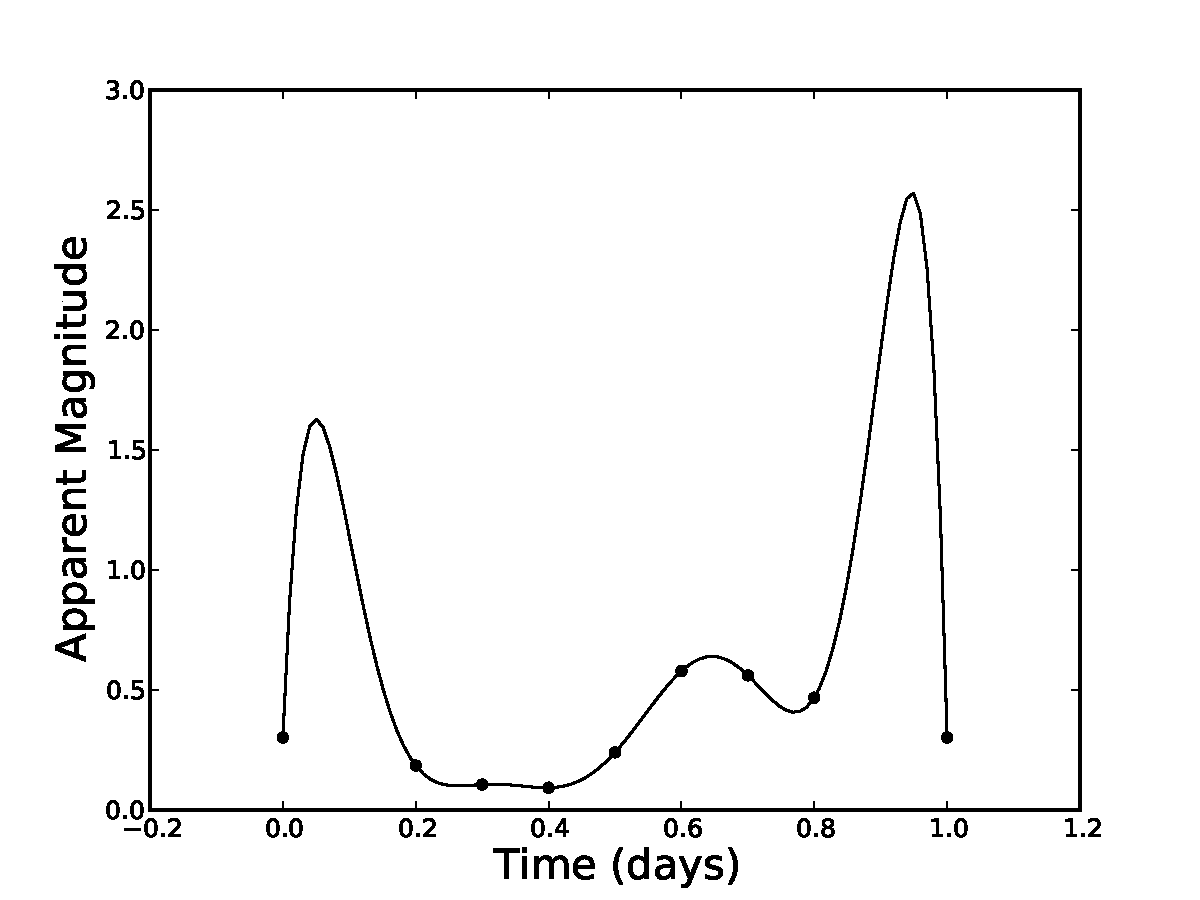
\includegraphics[width=0.5\textwidth]{foura.pdf}
\caption{Lagrange interpolation of the Cepheid lightcurve.  The 
points represent the data, while the solid curve represents 
the interpolated $p(x)$.  The 
interpolation looks reasonable in the middle, but exhibits Runge's 
phenomenon at the edges of the data.}
\label{fig:four}
\end{figure} 

\subsection{Part b}
I did not have time to do this part, although I expect that the 
interpolation will be more accurate since piecewise interpolation 
using low degree polynomials avoids the large oscillations of 
Runge's phenomenon.

\section{Problem Five}
\subsection{Part a}
I also did not have time for this part.  Again, since this is a 
piecewise interpolation, I expect the oscillations seen in the 
Lagrange interpolation to not be present.

\subsection{Part b}
I used Python's built in spline interpolator (scipy.interpolate.splrep) 
to do a natural cubic spline interpolation.  The result is shown 
Figure \ref{fig:five}.  Like the other piecewise methods, there are 
no large oscillations.  Figure \ref{fig:five2} shows the Lagrange 
and spline interpolations together for comparison.

\begin{figure}
\centering
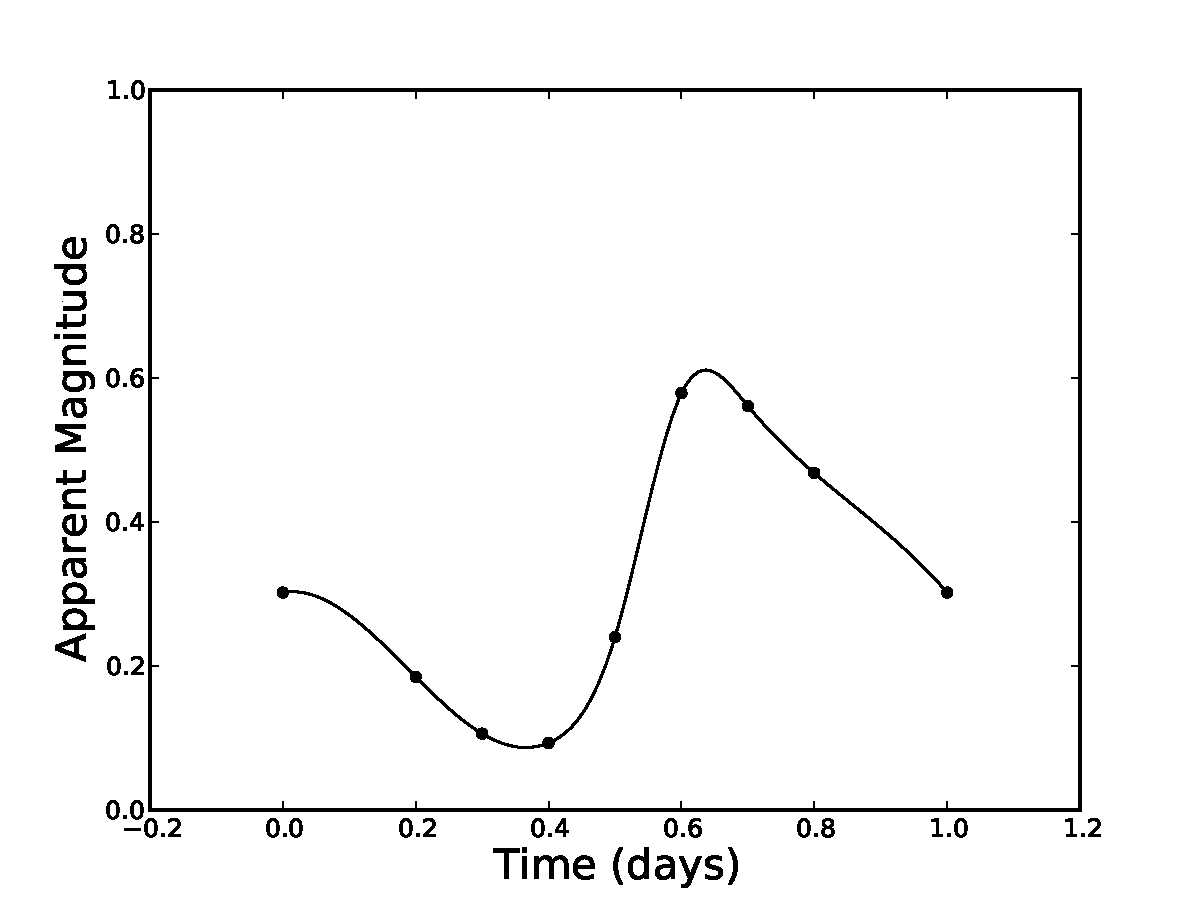
\includegraphics[width=0.5\textwidth]{fiveb.pdf}
\caption{Spline interpolation of the Cepheid light curve.  The 
points represent the data, while the solid curve represents 
the interpolated $p(x)$.  The 
oscillations seen in the Lagrange interpolation are not present.}
\label{fig:five}
\end{figure} 

\begin{figure}
\centering
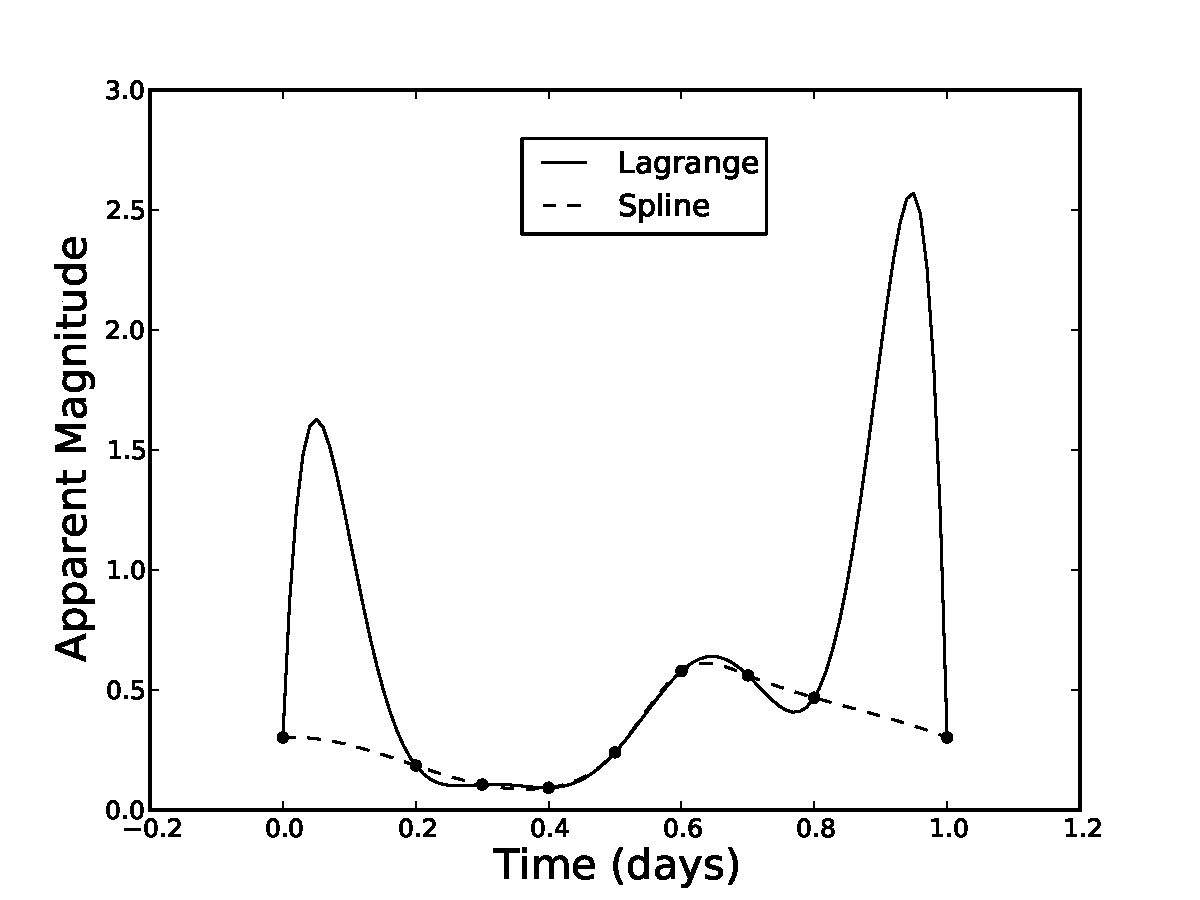
\includegraphics[width=0.5\textwidth]{five2.pdf}
\caption{Lagrange (solid line) and spline (dashed line) interpolations 
together, for comparison.  The solid points represent the data.}
\label{fig:five2}
\end{figure} 

\end{document}
Anything that comes after \end{document} is completely
ignored by LaTeX.
